%======================================================================
\chapter{Control Algorithm}
%======================================================================
To start the group wanted to create an algorithm that would monitor all devices on BEMOSS and use machine learning to optimize the consumer's behavior. To begin however we developed models for an HVAC system that could currently be controlled on BEMOSS but has no built in energy management support and a model of a motor that we developed to be controlled on BEMOSS. 
%----------------------------------------------------------------------
\section{System Modeling}
%----------------------------------------------------------------------
To develop our models we used Matlab and Simulink and created block diagram models for a HVAC system as well as a motor controlled using a PWM signal and H-bridge. To create realistic models we used a Simulink library, Simscape, that has built in electromechanical blocks that we can adjust the parameters of to better model our real world system.

\subsection{Motor}
The model of the motor was based on the initial design constraints of our hardware. 
\begin{figure}
    \centering
    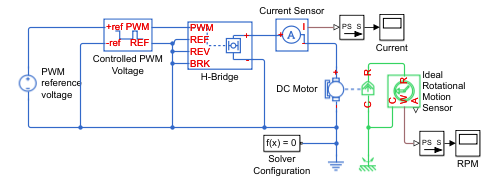
\includegraphics{figs/img/motorModelWithHBridge.png}
    \caption{Motor Model in Simulink}
    \label{fig:my_label}
\end{figure}
As can be noted the model is controlled witha  PWM signal and H-bridge that can be used to run the motor in clockwise and counterclockwise directions. A current sensor is used to read the current output so that the power calculation can be done later in the model. A rotational sensor reads the rotation of the motor in rotations per minute. The DC motor is based on the Pittman 24V DC motor we are currently controlling through BEMOSS in the lab. To do this a DC motor block from simscape is used and the specifications are defined as they appear in the Pittman datasheet. This allows an accurate reading, however it should be noted that the blocks used in Simulink are ideal blocks with no losses to friction or transmission losses. 
\subsection{HVAC Model}
\begin{figure}
    \centering
    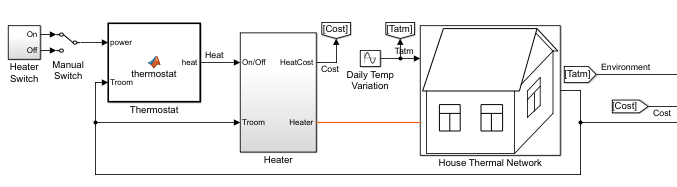
\includegraphics[scale = 0.85]{figs/img/houseModel.PNG}
    \caption{HVAC House Model}
    \label{fig:my_label}
\end{figure}
In this HVAC House Model in Figure 3.2, the thermal properties of a one room home is modeled. An on-off heating control is used to control the temperature of the house. A thermostat block is used to determine if the current temperature in the house model is below the reference signal and using this basic check switches the heating system on or off. The house model itself exchanges heat between three components: air to window, air to wall, and air to roof. This is a simple modeling that is used to show the typical behavior of a house, even if the house itself is not a real world object. The outside temperature is a fluctuating sine wave to determine if the simple on off control will handle changes in temperature. 

\subsection{State-Space Representation of HVAC System}
To better design a more realistic model the team looked at the works of \cite{Kang2014}. The design put forth by the team in \cite{Kang2014} is designed using a State-Space Representation. The typical control problem is defined as 
\begin{equation}
    \Dot{x} = Ax+Bu
\end{equation}
The system used in \cite{Kang2014} is a conventional HVAC system used in many buildings that controls temperature and humidity. In addition the system also measures and controls $CO_2$. 
\newline
To begin a conventional HVAC system that controls only temperature and humidity will be defined and later in the report, built upon to include $CO_2$ monitoring. 

\section{Control of HVAC Model}

%%% Local Variables:
%%% mode: latex
%%% TeX-master: "../finalReportMainV1"
%%% End:
